
 Yes. Any global minimum is also a local minimum. If the function
  is convex, a local minimum is
  also a global minimum. If not, there
  may be local minima that are not global. 
An example of such a function could be
$$f(x)=-2x^2 + x^4 - x^3.$$

\begin{center}
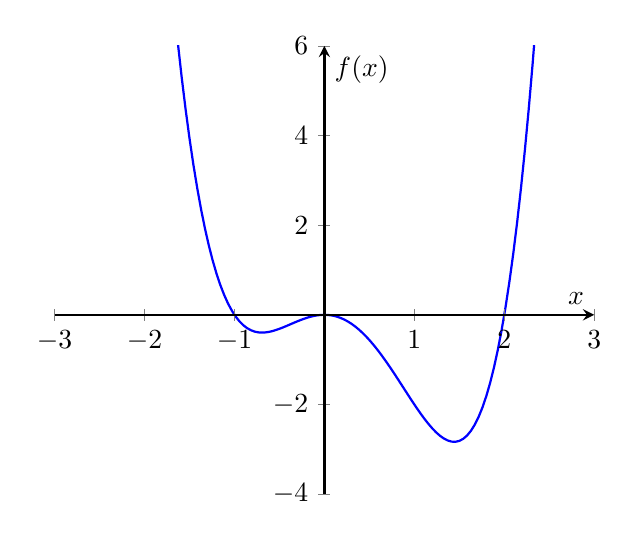
\begin{tikzpicture}
\begin{axis}[ xlabel={$x$}, ylabel={$f(x)$}
,axis on top=true
,axis lines=middle
,samples=141, thick,
,domain=-3:3, xmin=-3, xmax=3,
    ymin=-4, ymax=6,
]
\addplot+ [mark=none]{-2*x^2 + x^4 - x^3};
\end{axis}
\end{tikzpicture}
\end{center}
We use the optimality conditions to identify the  maxima and minima of
the function. The first derivative of $f(x)$ is
$$ f'(x)= -4x+4x^3-3x^2.$$
If we solve $f'(x)=0$, we obtain three solutions: $$x_1=0, \quad x_2=-0.693, \quad x_3=1.443.$$
These are the only candidates to be minima or maxima.
\begin{itemize}
\item Consider the interval $[-0.1,0.1]$. $x_1$ reaches the maximum of $f$
in this neighborhood. It is therefore a local maximum. 
\item Consider the interval $[-0.7,-0.6]$. $x_2$ reaches the minimum of $f$
in this neighborhood. It is therefore a local minimum. 
\item Consider the interval $[1.4,1.5]$. $x_3$ reaches the minimum of $f$
in this neighborhood. It is therefore a local minimum. 
\end{itemize}
This can also be verified using the second derivative of the function $f(x)$: 
$$f''(x)=-4+12x^2-6x.$$
Indeed, if we substitute the solutions $x$  in the function $f''(x)$ we obtain:
\begin{align*}
f''(x_1)=-4+12(0)^2-6(0)&=-4 &<   0 \Rightarrow & \text{local maximum},\\
f''(x_2)=-4+12(-0.693)^2-6(-0.693)&=5.92 &>  0 \Rightarrow &
\text{local minimum}, \\
f''(x_3)=-4+12(1.443)^2-6(1.443)&=12.32 &>  0 \Rightarrow &
\text{local minimum}.
\end{align*}
Since the function is a polynomial, we have
\begin{align*}
\lim_{x\to\infty} f(x)=& \lim_{x\to\infty} -2x^2 + x^4 - x^3= + \infty,\\
\lim\limits_{x\to -\infty} f(x)=& \lim\limits_{x\to -\infty} -2x^2 + x^4 - x^3=+ \infty.
\end{align*}
Therefore, the function has no global maximum.
Its global minimum is the local minimum associated with the lowest
value of $f$.
We can conclude that the function has
\begin{itemize}
\item a local maximum at $x_1=0$, $f(x_1)=0$, 
\item a local minimum at $x_2=-0.693$, $f(x_2)=-0.554$, and
\item a global minimum at $x_3=1.443$, $f(x_3)=-2.77$.
\end{itemize}

